\documentclass{beamer}
\usetheme{Copenhagen}
\usepackage[utf8]{inputenc}
\usepackage[spanish]{babel}
\usepackage{amsthm,amsmath,amsfonts,amssymb}
\usepackage{graphicx}
\usepackage{subcaption}
\usepackage{threeparttable}
\usepackage{multicol}
\newtheorem{definic}{Definición}[section]
\newtheorem{teorema}{Teorema}[section]

\newcommand\Wider[2][3em]{
\makebox[\linewidth][c]{
  \begin{minipage}{\dimexpr\textwidth+#1\relax}
  \raggedright#2
  \end{minipage}
  }
}


\title{Tipo de Cambio Real de Equilibrio para Bolivia}
\author{Hugo Pablo Rocha Portugal \and Paola Cecilia Yujra Tonconi}
\date{\today}


\begin{document}

\begin{frame}
\titlepage
\end{frame}

\begin{frame}{Contenido}
\begin{multicols}{2}
\tableofcontents
\end{multicols}
\end{frame}

\section[Introducción]{Introducción}
\subsection[Motivación]{Motivación}
\begin{frame}{Motivación}
¿Por qué es importante estudiar el TCR desde la perspectiva del equilibrio?
\begin{itemize}
\item Brinda nociones para encontrar el balance entre el denominado equilibrio interno y externo, lo que contribuye a determinar el desalineamiento que se refleja en el resultado de la balanza comercial   
\item Otorga información sobre el set de variables que influyen en la determinación del equilibrio.
\end{itemize}
\end{frame}

\begin{frame}{Motivación}
¿Por qué es relevante en el caso Boliviano?
\begin{itemize}
\item El sector externo es importante en la estructura de la economía, siendo pertinente estudiar las variables que la fomentan.
\item Teóricamente: Los incentivos a exportar pueden verse afectados frente a desalineamientos del TCR con relación a su nivel de equilibrio. 
\item Evidencia sugiere que los desalineamientos del TCR, tienen efectos negativos sobre el crecimiento.   
\end{itemize}
\end{frame}

\subsection[Consideraciones]{Consideraciones}
\begin{frame} {Consideraciones}
De acuerdo a la evidencia empírica.
\begin{itemize}
\item TCRE no es un número invariante y su valor se ve modificado frente al cambio de las variables que determinan su equilibrio interno y externo. 
\item Por lo tanto su valor será diferente para distintos momentos del ciclo económico, considerando además que es afectado por valores pasados y futuros de sus fundamentos
\item Su estimación, dependerá entonces de elecciones ``controversiales", que parten desde las definiciones de TCR y equilibrio.     
\end{itemize}
\end{frame}

\subsection[Definiciones]{Definiciones}
\begin{frame}{Definiciones}
\begin{definic}[Tipo de cambio real de equilibrio]
En una variable no observada y su valor se ve modificado frente al cambio de las variables que determinan su equilibrio interno y externo.
\end{definic}
\begin{definic}[Equilibrio Interno]
Se logra cuando los mercados internos de la economia local se encuentran en equilibrio.
\end{definic}
\begin{definic}[Equilibrio Externo]
Se alcanza cuando la trayectoria de la cuenta corriente es compatible con los flujos de capitales sostenibles a LP.
\end{definic}
\end{frame}

\section[BEER]{BEER}
\subsection[Metodología]{Metodología}
\begin{frame}{Definiciones}
\begin{definic}[BEER - Behavioral Equilibrium Exchange Rate]
TCRE se obtiene a partir de la estimación de una ecuación en su forma reducida. 
\begin{equation}\label{BEER}
q_t=\beta_1 z_1t + \beta_2 z_2t + \tau T_t + e_t
\end{equation}
\end{definic}
Donde: 
\begin{itemize}
\item $z_1$: Fundamentos económicos que se espera tengan efectos persistentes
\item $z_2$: Fundamentos económicos de los que se espera tengan efectos en el mediano plazo - coinciden con el ciclo económico
\item $T$: Vector de efectos transitorios en el CP
\item $e_t$: Término aleatorio
\end{itemize}
\end{frame}

\begin{frame}{Modelo de comportamiento}
Consideraciones
\begin{itemize}
\item Otorga un análisis dinámico de stock y flujos
\item El modelo, no lidia con el concepto de equilibrio interno y externo.
\item El enfoque no necesariamente considera elementos normativos o estructurales, por lo que la especificación carece de una adecuada identificación teórica
\item Montiel (1997), propone la especificación mediante modelos de equilibrio parcial para economías en desarrollo, que son estimados mediante VECM.
\end{itemize}
\end{frame}

\begin{frame}{Modelo de comportamiento}
Supuestos (Calderón, 2002; Montiel, 1997; Obstfeld \& Rogoff, 1995): 
\begin{enumerate}
\item Existen dos países el local y foráneo cada uno con 2 sectores de producción: Transable y No Transable
\item El S. Transable tiene un solo bien homogéneo determinado en los mercados internacionales de forma competitiva, No transable es monopólico con precios rígidos.  
\item Las preferencias sobre el consumo real y el esfuerzo laboral son similares para todos los agentes
\item El gobierno consume únicamente bienes no transables
\item El agente representativo doméstico puede invertir en un activo (bonos) transable internacional 
\end{enumerate}
\end{frame}

\subsection[Identificación]{Identificación}
\begin{frame}{Identificación}
\small{
\begin{align}
\ln TCR_t=&\phi_0+\phi_1\left(\frac{F}{Y}\right)_t+\phi_2\ln\left(\frac{Y_T}{A_N} / \frac{Y_T^*}{A_N^*}\right)_t+\phi_3\ln\left(\frac{P_T^X}{P_T^M}\right)_t\\\nonumber&+\phi_4\ln\left(\frac{G}{G^*}\right)_t+\mu_t
\end{align}
}
\begin{itemize}
\item $\phi_1<0$: Pasivos externos importantes, necesitan la generación de superavit (depreciación)
\item $\phi_2<0$, $\phi_4>0$: Productividad de transables crece más rápido en el país local que en el extranjero (apreciación)
\item $\phi_3<0$: Mejoras en los términos de intercambio se traduzcan en incremento de precios de bienes NT (apreciación)
\item $\phi_5<0$: Gasto de gobierno principalmente en no transables (apreciación)
\end{itemize}
\end{frame}

\subsection[Datos]{Datos}
\begin{frame}{Datos}
Información trimestral 1991q1 - 2017q3. A excepción de los términos de intercambio, el resto de varaibles son de elabroación propia.\\
Productividad:
\begin{enumerate}
\item Aproximada a partir del ratio de PIB per capita ponderado por la participación de comercio. 
\item Ratio entre precios transables y no transables de Bolivia. 
\item Ratio del índice de salario medio de sector transable y no transable
\end{enumerate}
\end{frame}

\begin{frame}{Datos}
Posición de activos externos netos:
\begin{enumerate}
\item Metodología de Lane y Milessi-Ferreti (2002), aproximación a partir del stock de deuda externa y reservas internacionales y el saldo de la CC. 
\item Aproximada por el saldo de CC.
\end{enumerate}
Gasto de gobierno:
\begin{enumerate}
\item Ratio del gasto de gobierno como porcentaje del PIB y el gasto de gobierno de los socios comercial en porcentaje a su PIB, ponderado por su participación en el comercio. 
\item Gasto de gobierno en no transables como porcentaje del PIB. 
\item Gasto de gobierno total como porcentaje del PIB.   
\end{enumerate}
\end{frame}

\begin{frame}
\begin{figure}
\captionsetup[subfigure]{font=scriptsize,labelfont=scriptsize}
\centering
    \begin{subfigure}[b]{0.4\textwidth}
        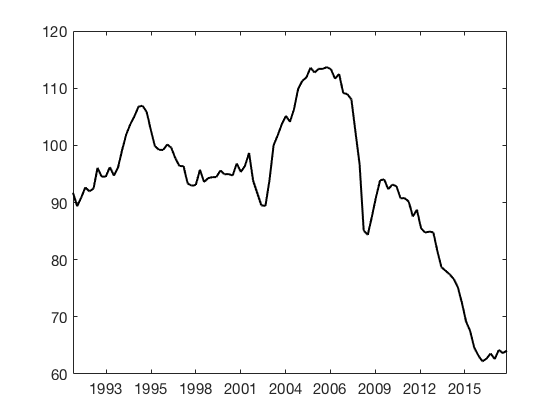
\includegraphics[width=\textwidth]{fig7}
        \caption{\tiny TCR}
    \end{subfigure}
    ~ %add desired spacing between images, e. g. ~, \quad, \qquad, \hfill etc. 
      %(or a blank line to force the subfigure onto a new line)
    \begin{subfigure}[b]{0.4\textwidth}
        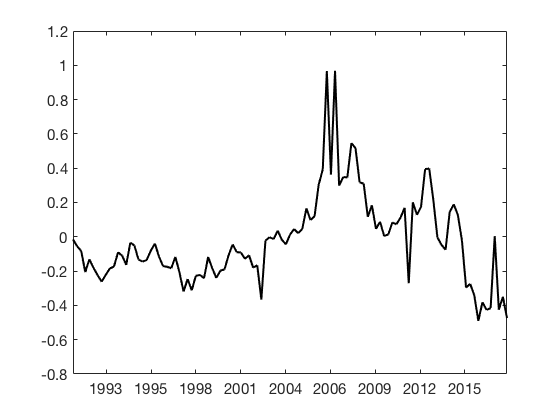
\includegraphics[width=\textwidth]{fig8}
        \caption{\tiny NFA}
    \end{subfigure}
    ~ %add desired spacing between images, e. g. ~, \quad, \qquad, \hfill etc. 
    %(or a blank line to force the subfigure onto a new line)
    \begin{subfigure}[b]{0.4\textwidth}
        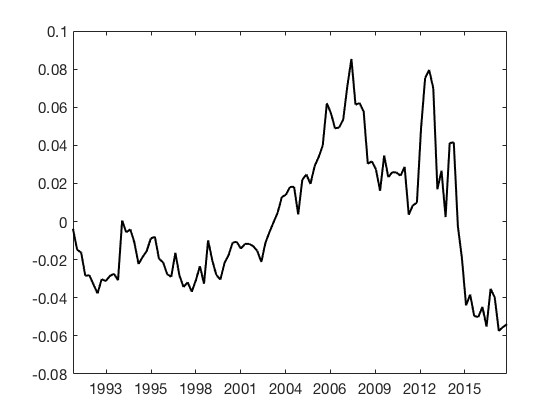
\includegraphics[width=\textwidth]{fig9}
        \caption{\tiny Saldo CC}
    \end{subfigure}
    ~ %add desired spacing between images, e. g. ~, \quad, \qquad, \hfill etc. 
    %(or a blank line to force the subfigure onto a new line)    
   \begin{subfigure}[b]{0.4\textwidth}
       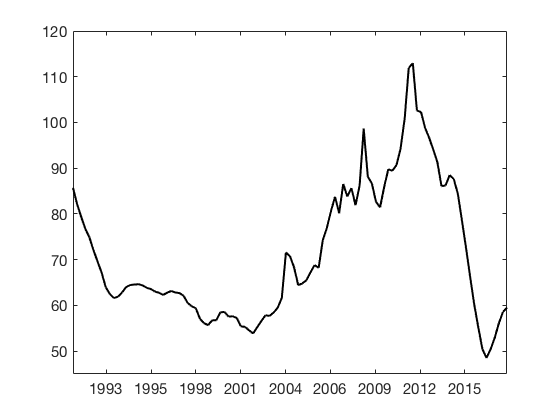
\includegraphics[width=\textwidth]{fig10}
        \caption{\tiny TI}
    \end{subfigure}
\end{figure}
\end{frame}

\begin{frame}
\begin{figure}
\captionsetup[subfigure]{font=scriptsize,labelfont=scriptsize}
\centering
    \begin{subfigure}[b]{0.4\textwidth}
       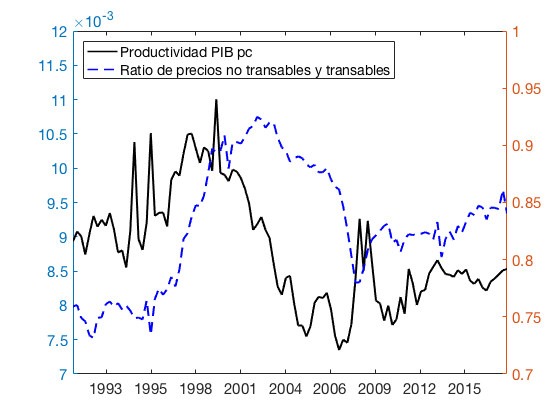
\includegraphics[width=\textwidth]{fig11}
        \caption{\tiny Productividad}
    \end{subfigure}
    ~ %add desired spacing between images, e. g. ~, \quad, \qquad, \hfill etc. 
      %(or a blank line to force the subfigure onto a new line)
    \begin{subfigure}[b]{0.4\textwidth}
        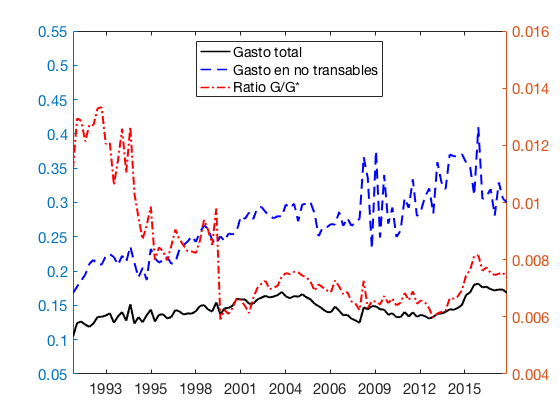
\includegraphics[width=\textwidth]{fig12}
        \caption{\tiny Gasto}
    \end{subfigure}
    ~ %add desired spacing between images, e. g. ~, \quad, \qquad, \hfill etc. 
    %(or a blank line to force the subfigure onto a new line)
    \begin{subfigure}[b]{0.4\textwidth}
        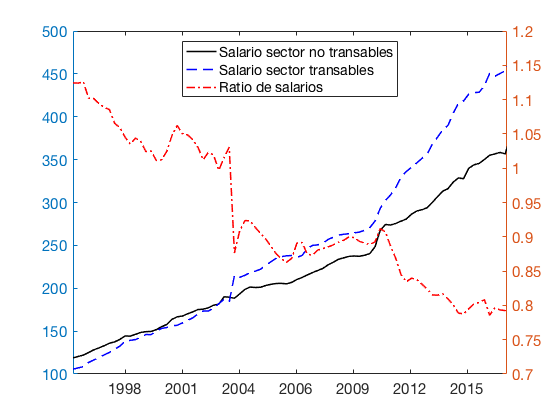
\includegraphics[width=\textwidth]{fig13}
        \caption{\tiny Salalarios}
    \end{subfigure}
\end{figure}
\end{frame}

%\begin{frame}{Correlaciones}
%\begin{figure}
%\captionsetup[subfigure]{font=scriptsize,labelfont=scriptsize}
%\centering
%    \begin{subfigure}[b]{0.31\textwidth}
%        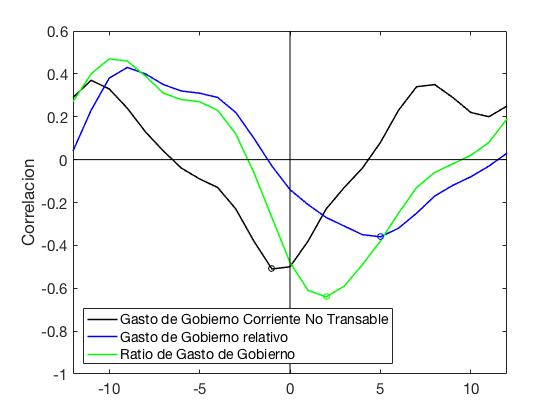
\includegraphics[width=\textwidth]{fig14}
%    \end{subfigure}
    ~ %add desired spacing between images, e. g. ~, \quad, \qquad, \hfill etc. 
      %(or a blank line to force the subfigure onto a new line)
%    \begin{subfigure}[b]{0.31\textwidth}
%        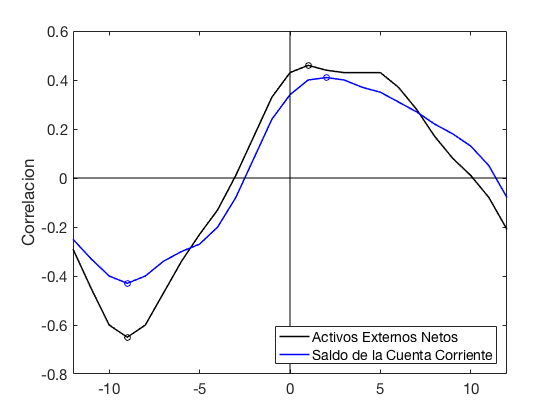
\includegraphics[width=\textwidth]{fig15}
%    \end{subfigure}
    ~ %add desired spacing between images, e. g. ~, \quad, \qquad, \hfill etc. 
    %(or a blank line to force the subfigure onto a new line)
%    \begin{subfigure}[b]{0.31\textwidth}
%        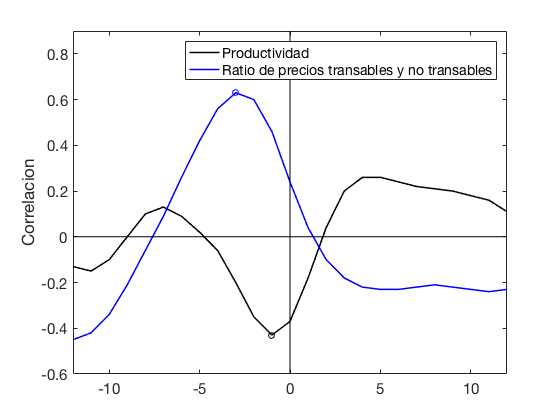
\includegraphics[width=\textwidth]{fig16}
%    \end{subfigure}
%   \begin{subfigure}[b]{0.31\textwidth}
%       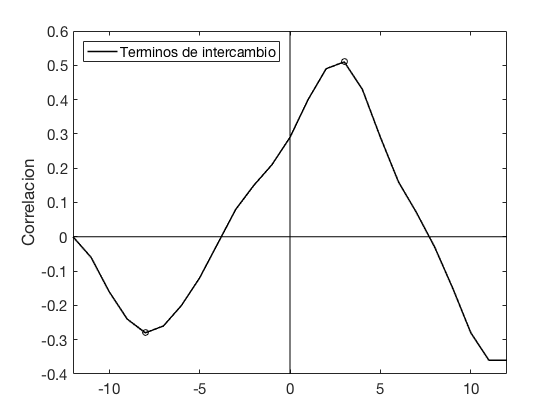
\includegraphics[width=\textwidth]{fig17}
%    \end{subfigure}
        ~ %add desired spacing between images, e. g. ~, \quad, \qquad, \hfill etc. 
    %(or a blank line to force the subfigure onto a new line)    
%   \begin{subfigure}[b]{0.31\textwidth}
%       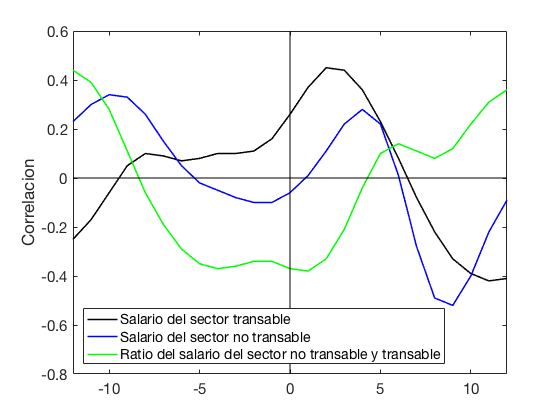
\includegraphics[width=\textwidth]{fig18}
%    \end{subfigure}
%\end{figure}
%\end{frame}

\subsection[Resultados]{Resultados}
\begin{frame}{Estimación del TCR: BEER}
\begin{table}
\begin{center}
\begin{threeparttable}
\scalebox{0.5}{
\begin{tabular}{lcccc}									
\hline									
\hline									
	&	Modelo 1	&	Modelo 2 V1	&	Modelo 2 V2	&	Modelo 3	\\
Variable	&	ln(TCR)	&	ln(TCR)	&	ln(TCR)	&	ln(TCR)	\\
	&	1	&	1	&	0	&	1	\\
\hline									\\
Constante	&	4,239	&	3,323	&	-3,897	&	4,576	\\
ln(GCNT/Y)	&	-0,803	&	&	&	\\
	&	(0,138)	&		&		&		\\
ln(G/Y) &		&	0	&	-1	&	-1,580**	\\
	&		&		&		&	(0,321)	\\
AEN/Y	&	0,741**	&		&		&		\\
	&	(-7,428)	&		&		&		\\
SCC/Y	&		&	6,172**	&	-1,106	&	7,236**	\\
	&		&	(0,650)	&	(0,253)	&	(1,035)	\\
ln(PNT/PT)	&	0,904**	&	0,554	&	0,452**	&		\\
	&	(0,128)	&	(0,327)	&	(0,127)	&		\\
ln(PIBpc/PIBpc*)	&		&	-0,851**	&	-0,622**	&	-0,566	\\
	&		&	(0,233)	&	(0,091)	&	(0,374)	\\
ln(PX/PM)	&	-0,137*	&	-0,645	&	-0,207	&	-1,364*	\\
	&	(0,128)	&	(0,116)	&	(0,045)	&	(0,218)	\\
ln(WNT/WT)	&		&	0,622**	&	-0,005	&		\\
	&		&	(0,195)	&	(0,076)	&		\\
\hline							
\hline									
\end{tabular}
}	
\begin{tablenotes}
\item \scriptsize  \emph{Nota.} La significancia al uno, cinco y diez por ciento es indicada\\ por ***, ** y *, respectivamente. El modelo 2 usa información \\trimestral desde 1996.I hasta 2017.I.
\end{tablenotes}								
\end{threeparttable}					
\end{center}
\end{table}	
\end{frame}

\begin{frame}
\begin{figure}
\centering
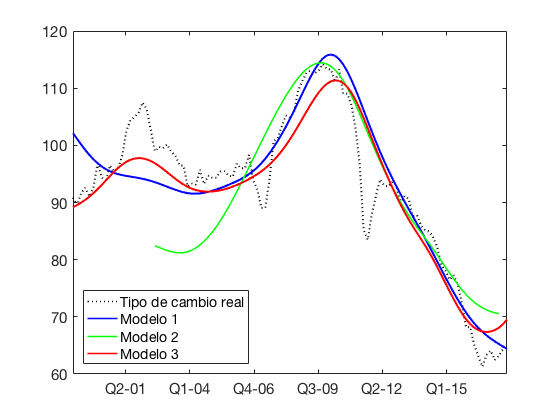
\includegraphics[width=\textwidth]{fig19}
\end{figure}
\end{frame}

\section[DEER]{DEER}
\subsection[Metodología]{Metodología}
\begin{frame}{FEER}
\begin{itemize}
\item Los modelos FEER están basados en el trabajo de Artis y Taylor (1995), Barrell y Wren-Lewis (1989) y Williamson (1993, 1994). Las modificaciones más modernas son de Bussiere (2003).
\item Generalmente se utilizan distintas metodologías para encontrar las normas y subyacentes de cuenta corriente. 
\item Dependiendo del objetivo se escogerá el mejor método.
\item Los más estudiados son el balance macroeconómico y la sostenibilidad externa.
\end{itemize}
\end{frame}

\begin{frame}{DEER}
\begin{itemize}
\item Los modelos DEER son menos normativos en el sentido de su elección de normas y objetivos de cuenta corriente.
\item DEER utilizará el equilibrio más probable de la economía, a diferencia de su versión normativa.
\item En cierta forma está condicionado por su factibilidad fiscal. 
\end{itemize}
\end{frame}

\subsection[Identificación]{Identificación}
\begin{frame}{Identificación}
\begin{definic}[Cuenta Corriente]
\begin{equation}\label{CC}
CC\equiv(P_XX-P_MM)+Ing1+Ing2
\end{equation}
\begin{equation}\label{cc}
cc=\frac{CC}{PIB}=\frac{BC}{PIB}+\frac{Ing1}{PIB}+\frac{Ing2}{PIB}
\end{equation}
\end{definic}
\begin{equation}\label{sup}
\frac{\partial CC}{\partial Q}=\frac{\partial BC}{\partial Q}
\end{equation}
Suponiendo $\frac{\partial Ing1}{\partial Q}=0$, $\frac{\partial Ing2}{\partial Q}=0$ y $\frac{\partial CC}{\partial Q}\approx \frac{\Delta CC}{\Delta Q}=CC-\bar{CC}$
\begin{equation}\label{dc}
\frac{\partial cc}{\partial Q}=cc-\bar{cc}
\end{equation}
\end{frame}

\begin{frame}{Identificación}
Si:
\begin{equation}\label{X}
X=f(\overset{+}{Y^*},\overset{+}{Q})
\end{equation}
\begin{equation}\label{M}
M=g(\overset{+}{Y},\overset{-}{Q})
\end{equation}
Entonces:
\begin{equation}
bc=\frac{P_X X}{PIB}-\frac{P_M M}{PIB}.
\end{equation}
\begin{equation}
\frac{\partial bc}{\partial Q}=\frac{\partial X}{\partial Q} \frac{P_X}{PIB}+\frac{\partial P_X}{\partial Q} \frac{X}{PIB} - \frac{\partial M}{\partial Q} \frac{P_M}{PIB}-\frac{\partial P_M}{\partial Q}\frac{M}{PIB},
\end{equation}
Donde: $\frac{\partial P_X}{\partial Q}=0$ y $\frac{\partial P_M}{\partial Q}=-\frac{P_M}{Q}$. Entonces:
\begin{equation}\label{partialq}
\frac{\partial bc}{\partial Q}=\frac{1}{Q} \left[\eta_X \frac{P_X X}{PIB}-(\eta_M -1)\frac{P_M M}{PIB}\right].
\end{equation}
\end{frame}

\begin{frame}{Identificación}
\begin{equation}
\frac{\partial cc}{\partial Q}=\frac{\partial bc}{\partial Q}
\end{equation}
\begin{equation}
Q^{FEER}=\frac{1}{cc-\bar{cc}}\left[\eta_X \frac{P_X X}{PIB}-(\eta_M -1)\frac{P_M M}{PIB}\right].
\end{equation}
\end{frame}

\subsection[Datos]{Datos}
\begin{frame}{Datos}
\begin{figure}
\captionsetup[subfigure]{font=scriptsize,labelfont=scriptsize}
\centering
    \begin{subfigure}[b]{0.31\textwidth}
        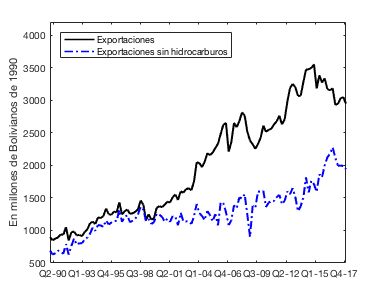
\includegraphics[width=\textwidth]{10exp}
        \caption{Exportación}
    \end{subfigure}
    ~ %add desired spacing between images, e. g. ~, \quad, \qquad, \hfill etc. 
      %(or a blank line to force the subfigure onto a new line)
    \begin{subfigure}[b]{0.31\textwidth}
        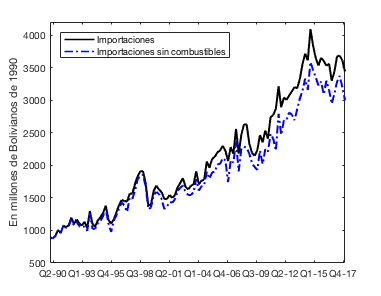
\includegraphics[width=\textwidth]{11imp}
        \caption{Importación}
    \end{subfigure}
    ~ %add desired spacing between images, e. g. ~, \quad, \qquad, \hfill etc. 
    %(or a blank line to force the subfigure onto a new line)
    \begin{subfigure}[b]{0.31\textwidth}
        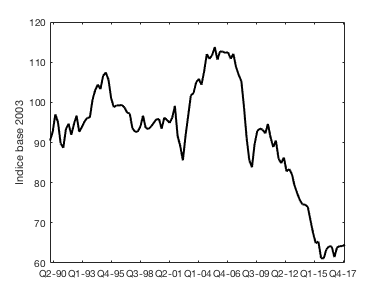
\includegraphics[width=\textwidth]{12tcr}
        \caption{TCR}
    \end{subfigure}
    \begin{subfigure}[b]{0.31\textwidth}
        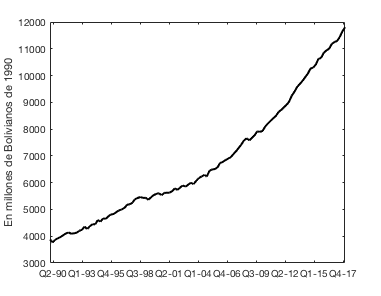
\includegraphics[width=\textwidth]{13pib}
        \caption{PIB}
    \end{subfigure}
    ~ %add desired spacing between images, e. g. ~, \quad, \qquad, \hfill etc. 
      %(or a blank line to force the subfigure onto a new line)
    \begin{subfigure}[b]{0.31\textwidth}
        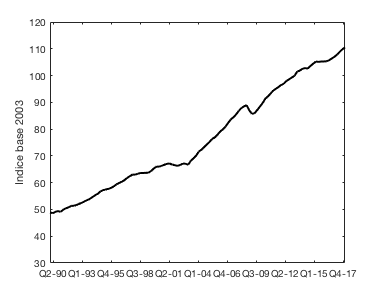
\includegraphics[width=\textwidth]{14pieb}
        \caption{PIB externo relevante}
    \end{subfigure}
    ~ %add desired spacing between images, e. g. ~, \quad, \qquad, \hfill etc. 
      %(or a blank line to force the subfigure onto a new line)
    \begin{subfigure}[b]{0.31\textwidth}
        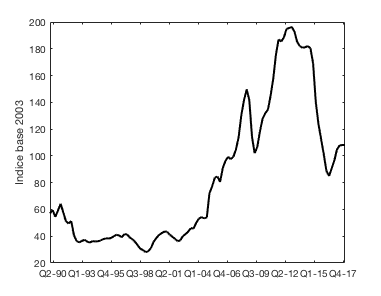
\includegraphics[width=\textwidth]{15ippbx}
        \caption{Precios internacionales}
    \end{subfigure}
\end{figure}
\end{frame}

\begin{frame}{Cuenta Corriente}
\begin{figure}
\centering
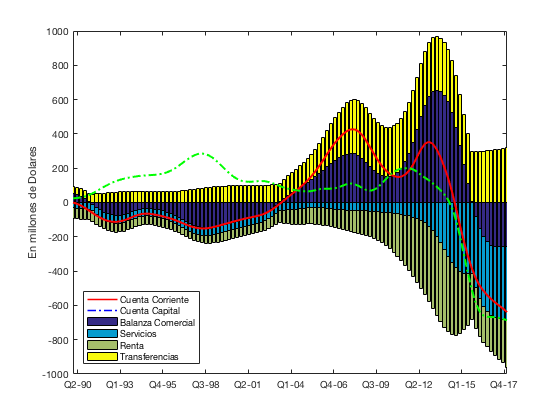
\includegraphics[scale=0.4]{cc}
\end{figure}
\end{frame}

\begin{frame}{Matriz de correlación}
\begin{table}
\begin{center}
\begin{threeparttable}
\scalebox{0.6}{
\begin{tabular}{lcccccc}									
\hline													
\hline												
	&	Exportaciones	&	Importaciones	&	PIB externo	&	TCR	&	IPPBX	&	PIB	\\
\hline													
Exportaciones	&	1	&		&		&		&		&		\\
Importaciones	&	0.9384	&	1	&		&		&		&		\\
PIB externo	&	0.9424	&	0.9751	&	1	&		&		&		\\
TCR	&	-0.5185	&	-0.7131	&	-0.7103	&	1	&		&		\\
IPPBX	&	0.8949	&	0.8506	&	0.8743	&	-0.3589	&	1	&		\\
PIB	&	0.9017	&	0.9645	&	0.9835	&	-0.8102	&	0.7821	&	1	\\
\hline													
\hline									
\end{tabular}	
}						
\begin{tablenotes}
\small
\item Elaboración propia.
\end{tablenotes}	
\end{threeparttable}
\end{center}
\end{table}	
\end{frame}

\subsection[Resultados]{Resultados}
\begin{frame}{Ecuaciones de comercio}
\begin{table}
\begin{center}
\begin{threeparttable}
\scalebox{0.45}{
\begin{tabular}{lcccccccccccc}									
\hline									
\hline	
					&	(1)				& (2) 			& (3)				& (4)				&	(5)			& (6)				&	(7) 					&	(8)					& (9)				& (10)			& (11)				& (12)\\
					&	$x$			& $x$ 			& $x_{sc}$	& $x_{sc}$	&	$\Delta x$	& $\Delta x$	& $\Delta x_{sc}$	&	$\Delta x_{sc}$	& $m$			& $m_{sc}$ 	& $\Delta m$ & $\Delta m_{sc}$\\
\hline	
$y^*$			&	1,511***	& 1,670***	& 1,750***	& 1,233***	&					&					&							&							&					&					&						&				\\
					&	(0.044)		& (0,024) 		& (0,051)		& (0,039)		&					&					&							&							&					&					&						&				\\
$\Delta y^*$	&					&					&					&					&	1,117*		& 1,369**		& 1,296					& 0,739				&					&					&						&				\\
					&					&					&					&					&	(0,613)		& (0,585)		& (1,039)				& (0,996)				&					&					&						&				\\
$y$				&					&					&					&					&					&					&							&							& 1,060*** 	& 1,010***	&						&				\\
					&					&					&					&					&					&					&							&							& (0,018)		& (0,017)		&						&				\\
$\Delta y$		&					&					&					&					&					&					&							&							&					&					& 1,088**			& 0,710		\\
					&					&					&					&					&					&					&							&							&					&					& (0,479)			& (0,568)	\\
$tcr$			&	0,133***	& 0,072***	& 0,207***	& 0,403***	&					&					&							&							& -0,384***	& -0,302***	&						&				\\
					&	(0,026)		& (0,023) 		& (0,030)		& (0,037)		&					&					&							&							& (0,036)		& (0,032)		&						&				\\
$\Delta tcr$	&					&					&					&					&	0,384*		& 0,362*		& 0,712**				& 0,760**				&					&					& -0,174			& -0,266	\\
					&					&					&					&					&	(0,195)		& (0,195)		& (0,330)				& (0,332)				&					&					& (0,235)			& (0,279)	\\
$P_X$			&	0,097***	&					& -0,316***	&					&					&					&							&							&					&					&						&				\\
					&	(0,023)		&					& (0,027)		&					&					&					&							&							&					&					&						&				\\
$\Delta P_X$	&					&					&					&					&	0,109		&					& -0,242*				&							&					&					&						&				\\
					&					&					&					&					&	(0,083)		&					& (0,141)				&							&					&					&						&				\\
\hline									
\hline									
\end{tabular}
}	
\begin{tablenotes}
\small
\item  \emph{Nota.} La significancia al uno, cinco y diez por ciento \\ es indicada por ***, ** y *, respectivamente.
\end{tablenotes}								
\end{threeparttable}					
\end{center}
\end{table}	
\end{frame}

\begin{frame}
\begin{figure}
\centering
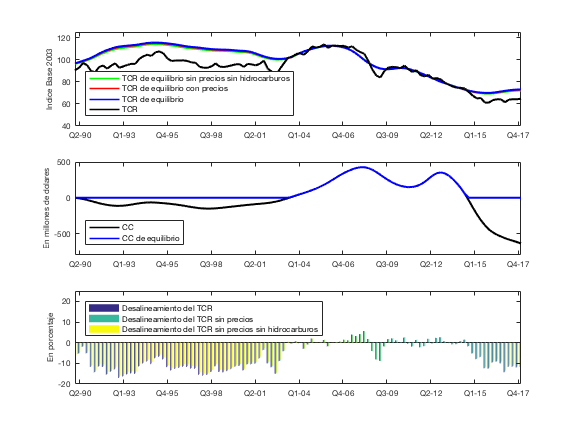
\includegraphics[scale=0.5]{deer}
\end{figure}
\end{frame}

\section[Política]{Política}
\begin{frame}{Si existe pass-through}
Dependiendo del nivel de \emph{pass-through}, considérese:
\begin{equation}
Q_t=E_t\frac{P_t^*}{P_t(E_t)},
\end{equation}
Donde, en niveles de \emph{pass-through} completos el tipo de cambio real únicamente depende del nivel de precios externo.
\end{frame}
\end{document}
